\frame
{
	\frametitle{Minimize the Number of Paths}
	{\bf Problem:} Given a DAG $G=(V,E)$ with single source $s$ and single sink $t$, 
		to compute a set of paths $\mathcal{P}$ with minimum cardinality
		that can cover all edges.

	\vspace{0.4cm}

	\begin{center}

\begin{tikzpicture}[font=\small,overlay,
mycirclex/.style={draw, circle, minimum size=1.0em, inner sep = 0.2mm}, 
mydiamond/.style={draw, diamond, minimum size=0.78em, inner sep = 0mm}, 
myrectang/.style={draw, rectangle, minimum size=0.60em, inner sep = 0mm}, 
>=stealth]

\definecolor{mygreen}{rgb}{0, 0.7, 0}
\definecolor{myyellow}{rgb}{0.8, 0.6, 0}

\def\colx{black}
\def\cola{red} 
\def\colb{blue}
\def\colc{violet}
\def\cold{cyan} 
\def\cole{myyellow}
\def\colf{brown}


\def\len{1.8cm}

% G1
\begin{scope}[local bounding box=bbox, xshift=-6.4cm]
\path<1-> node[mycirclex] (v1) at (1.0 * \len, 0) {$s$};
\path<1-> node[mycirclex] (v2) at (2.0 * \len, 0) {$a$};
\path<1-> node[mycirclex] (v3) at (3.0 * \len, 0) {$b$};
\path<1-> node[mycirclex] (v4) at (4.0 * \len, 0) {$c$};
\path<1-> node[mycirclex] (v5) at (5.0 * \len, 0) {$d$};

\path<1-> [draw, \colx, ->, line width=0.04cm] (v1) -- (v2);
\path<1-> [draw, \colx, ->, line width=0.04cm] (v2) -- (v3);
\path<1-> [draw, \colx, ->, line width=0.04cm] (v3) -- (v4);
\path<1-> [draw, \colx, ->, line width=0.04cm] (v4) -- (v5);

\path<1-> [draw, \colx, ->, line width=0.04cm, bend left = 40] (v1) to (v3);
\path<1-> [draw, \colx, ->, line width=0.04cm, bend left = 27] (v2) to (v5);
\path<1-> [draw, \colx, ->, line width=0.04cm, bend left =-40] (v2) to (v4);

\path<1-> node at (1.5 * \len, 0.18cm) {$e_1$};
\path<1-> node at (2.5 * \len, 0.18cm) {$e_2$};
\path<1-> node at (3.5 * \len, 0.18cm) {$e_3$};
\path<1-> node at (4.5 * \len, 0.18cm) {$e_4$};

\path<1-> node at (2.0 * \len, 0.9cm) {$e_5$};
\path<1-> node at (3.0 * \len,-0.6cm) {$e_6$};
\path<1-> node at (3.5 * \len, 0.9cm) {$e_7$};

\end{scope}
%\path<1-> [draw, rounded corners] ($(bbox.south west) - (0.00cm, 0.25cm)$) rectangle ($(bbox.north east) + (0.1cm, 0)$);
%\node at ($(bbox.south) - (0.00cm, 0.2cm)$) [label=below:{$G_2 - G_1 = \{c\}$}]{};


\end{tikzpicture}
\end{center}


	\vspace{0.6cm}

	\onslide<2->{{\bf Polynomial-time Algorithm}}
	\vspace{-0.2cm}
	\begin{center}

\begin{tikzpicture}[font=\small,overlay,
mycirclex/.style={draw, circle, minimum size=1.0em, inner sep = 0.2mm}, 
mydiamond/.style={draw, diamond, minimum size=0.78em, inner sep = 0mm}, 
myrectang/.style={draw, rectangle, minimum size=0.60em, inner sep = 0mm}, 
>=stealth]

\definecolor{mygreen}{rgb}{0, 0.7, 0}
\definecolor{myyellow}{rgb}{0.8, 0.6, 0}

\def\colx{black}
\def\cola{red} 
\def\colb{blue}
\def\colc{violet}
\def\cold{cyan} 
\def\cole{myyellow}
\def\colf{brown}


\def\len{1.2cm}

% G1
\begin{scope}[local bounding box=bbox, xshift=-5.5cm]
\path<2-> node[mycirclex] (x1) at (1.0 * \len, 0.0) {$e_1$};
\path<2-> node[mycirclex] (x2) at (2.0 * \len, 0.0) {$e_2$};
\path<2-> node[mycirclex] (x3) at (3.0 * \len, 0.0) {$e_3$};
\path<2-> node[mycirclex] (x4) at (4.0 * \len, 0.0) {$e_4$};
\path<2-> node[mycirclex] (x5) at (5.0 * \len, 0.0) {$e_5$};
\path<2-> node[mycirclex] (x6) at (6.0 * \len, 0.0) {$e_6$};
\path<2-> node[mycirclex] (x7) at (7.0 * \len, 0.0) {$e_7$};

\path<2-> node[mycirclex] (y1) at (1.0 * \len, -2.0) {$e_1$};
\path<2-> node[mycirclex] (y2) at (2.0 * \len, -2.0) {$e_2$};
\path<2-> node[mycirclex] (y3) at (3.0 * \len, -2.0) {$e_3$};
\path<2-> node[mycirclex] (y4) at (4.0 * \len, -2.0) {$e_4$};
\path<2-> node[mycirclex] (y5) at (5.0 * \len, -2.0) {$e_5$};
\path<2-> node[mycirclex] (y6) at (6.0 * \len, -2.0) {$e_6$};
\path<2-> node[mycirclex] (y7) at (7.0 * \len, -2.0) {$e_7$};

\path<3-> [draw, \cola, line width=0.08cm] (x1) -- (y2);
\path<3-> [draw, \cola, line width=0.08cm] (x2) -- (y3);
\path<3-> [draw, \cola, line width=0.08cm] (x5) -- (y4);

\path<2-> [draw, \colx, line width=0.03cm] (x1) -- (y2);
\path<2-> [draw, \colx, line width=0.03cm] (x1) -- (y3);
\path<2-> [draw, \colx, line width=0.03cm] (x1) -- (y4);
\path<2-> [draw, \colx, line width=0.03cm] (x1) -- (y6);
\path<2-> [draw, \colx, line width=0.03cm] (x1) -- (y7);
\path<2-> [draw, \colx, line width=0.03cm] (x2) -- (y3);
\path<2-> [draw, \colx, line width=0.03cm] (x2) -- (y4);
\path<2-> [draw, \colx, line width=0.03cm] (x3) -- (y4);
\path<2-> [draw, \colx, line width=0.03cm] (x5) -- (y3);
\path<2-> [draw, \colx, line width=0.03cm] (x5) -- (y4);
\path<2-> [draw, \colx, line width=0.03cm] (x6) -- (y4);

\end{scope}
%\path<2-> [draw, rounded corners] ($(bbox.south west) - (0.00cm, 0.25cm)$) rectangle ($(bbox.north east) + (0.1cm, 0)$);
%\node at ($(bbox.south) - (0.00cm, 0.2cm)$) [label=below:{$G_2 - G_1 = \{c\}$}]{};


\end{tikzpicture}
\end{center}


	\vspace{2.0cm}
	\onslide<3->{$|\mathcal{P}| = |E| - M$, where $M$ is the size of one maximum matching.}
}

\frame
{
	\frametitle{Open Problems}
	\begin{itemize}
	\item Design approximation algorithms with the constraint that every edge has to be covered.
	\end{itemize}
}

\frame
{
	\frametitle{Existing Method: Cufflinks}

	\begin{itemize}
	\item {\bf Algorithm:} compute a minimum number of paths to cover all edges using Dilworth's Theorem
	\vspace{0.5cm}
	\item {\bf Disadvantage:} do not consider the weights of edges
	\end{itemize}
}

\frame
{
	\frametitle{Existing Method: Scripture}
	\begin{itemize}
	\item {\bf Algorithm:} output all possible paths
	\vspace{0.5cm}
	\item {\bf Disadvantage:} exponential number of paths
	\end{itemize}
}


\frame
{
	\frametitle{Existing Method: IsoLasso}
	\begin{itemize}
	\item {\bf Algorithm:} use quadratic programming
		\begin{displaymath}
		\begin{array}{rl}
		\min & \sum_{e\in E} | w(e) - \sum_{e\in P} c(P)|^2 \\
		\textrm{s.t.} & \sum_{P\in\mathcal{P}} c(P) \le \lambda
		\end{array}
		\end{displaymath}

	\vspace{0.2cm}
	\item {\bf Disadvantage:} 
		\begin{itemize}
		\item $|\mathcal{P}|$ is not bounded
		\item exponential number of variables
		\end{itemize}

	\end{itemize}
}


\frame
{
	\frametitle{Existing Method: Traph}
	\begin{itemize}
	\item {\bf Algorithm:} use a network flow formulation to compute a new
		weight $w'(e)$ for $e\in E$ such that
		\begin{itemize}
		\item $\sum_{e\in E} |w(e) - w'(e)|$ is minimized, and that 
		\item there exists a flow decompositions of the new DAG, i.e.,
		there \emph{exists} a set of paths satisfying $\sum_{e\in E} | w'(e) - \sum_{e\in P} c(P)| = 0$
		\end{itemize}
	\vspace{0.4cm}
	\item {\bf Disadvantage:} 
		\begin{itemize}
		\item only the weights are updated; the paths are not returned; actually
			they use a greedy algorithm to compute paths~(the same as StringTie)
		\vspace{0.2cm}
		\item the number of paths is not considerred in this formulation
		\end{itemize}
	\end{itemize}
}

\frame
{
	\frametitle{Existing Method: CLIIQ}
	\begin{itemize}
	\item {\bf Algorithm:} use ILP to model this problem
	\vspace{0.5cm}
	\item {\bf Disadvantage:} 
		\begin{itemize} 
		\item ILP itself is NP-complete
		\item exponential number of variables
		\end{itemize}
	\end{itemize}
}

\frame
{
	\frametitle{Existing Method: StringTie}
	\begin{itemize}
	\item {\bf Algorithm:} 
		\begin{itemize}
		\item use greedy algorithm to compute paths~(transcripts): iteratively
			compute heaviest path
		\item use network flow formulation to estimate abundance~(a sophisticated
				way to handle reads spanning several vertices)
		\end{itemize}
	\vspace{0.5cm}
	\item {\bf Disadvantage:} 
		\begin{itemize} 
		\item when compute the current path, the tradeoff between weights is
			not considerred
		\end{itemize}
	\end{itemize}
}

\frame
{
	\frametitle{Our Algorithm}
	\begin{enumerate}
	\item compute a (good) basis $\mathcal{B}$~(with $|E|-|V|+2$ paths) of the path space
	\vspace{0.2cm}
	\item use an LP to estimate the capacities of the paths in $\mathcal{B}$
	\vspace{0.2cm}
	\item try to reduce the number of paths in $\mathcal{B}$
		\begin{itemize}
		\vspace{0.1cm}
		\item for two paths with (almost) identical capacities, merge them into one path
		\vspace{0.1cm}
		\item discard paths with very small capacities
		\end{itemize}
	\vspace{0.2cm}
	\item iterate between step 2 and step 3
	\end{enumerate}
}

\frame
{
	\frametitle{Compute Basis of the Path Space}

	\begin{enumerate}
	\item for each vertex~(except $s$ and $t$), arbitrarily choose exactly an in-edge and an out-edge~(the one with maximum weight);
	\vspace{1.2cm}
	\begin{center}

\begin{tikzpicture}[font=\small,overlay,
mycirclex/.style={draw, circle, minimum size=1.0em, inner sep = 0.2mm}, 
mydiamond/.style={draw, diamond, minimum size=0.78em, inner sep = 0mm}, 
myrectang/.style={draw, rectangle, minimum size=0.60em, inner sep = 0mm}, 
>=stealth]

\definecolor{mygreen}{rgb}{0, 0.7, 0}
\definecolor{myyellow}{rgb}{0.8, 0.6, 0}

\def\colx{black}
\def\cola{red} 
\def\colb{blue}
\def\colc{violet}
\def\cold{cyan} 
\def\cole{myyellow}
\def\colf{brown}


\def\len{1.8cm}

% G1
\begin{scope}[local bounding box=bbox, xshift=-6.4cm]
\path<1-> node[mycirclex] (v1) at (1.0 * \len, 0) {$s$};
\path<1-> node[mycirclex] (v2) at (2.0 * \len, 0) {$a$};
\path<1-> node[mycirclex] (v3) at (3.0 * \len, 0) {$b$};
\path<1-> node[mycirclex] (v4) at (4.0 * \len, 0) {$c$};
\path<1-> node[mycirclex] (v5) at (5.0 * \len, 0) {$d$};
\path<1-> node[mycirclex] (v6) at (6.0 * \len, 0) {$t$};

\path<1-> [draw, \cola, ->, line width=0.10cm] (v3) -- (v4);
\path<1-> [draw, \cola, ->, line width=0.10cm] (v4) -- (v5);

\path<1-> [draw, \cola, ->, line width=0.04cm] (v1) -- (v2);
\path<1-> [draw, \colx, ->, line width=0.04cm] (v2) -- (v3);
\path<1-> [draw, \colb, ->, line width=0.04cm] (v3) -- (v4);
\path<1-> [draw, \colb, ->, line width=0.04cm] (v4) -- (v5);
\path<1-> [draw, \colb, ->, line width=0.04cm] (v5) -- (v6);

\path<1-> [draw, \cola, ->, line width=0.04cm, bend left = 40] (v1) to (v3);
\path<1-> [draw, \colb, ->, line width=0.04cm, bend left =-40] (v2) to (v5);
\path<1-> [draw, \colx, ->, line width=0.04cm, bend left = 40] (v3) to (v5);
\path<1-> [draw, \colx, ->, line width=0.04cm, bend left =-40] (v4) to (v6);

\path<1-> node at (1.5 * \len, 0.2cm) {$4$};
\path<1-> node at (2.5 * \len, 0.2cm) {$1$};
\path<1-> node at (3.5 * \len, 0.2cm) {$5$};
\path<1-> node at (4.5 * \len, 0.2cm) {$4$};
\path<1-> node at (5.5 * \len, 0.2cm) {$9$};

\path<1-> node at (2.0 * \len, 1.0cm) {$6$};
\path<1-> node at (4.0 * \len, 1.0cm) {$2$};
\path<1-> node at (5.0 * \len,-1.0cm) {$1$};
\path<1-> node at (3.5 * \len,-1.3cm) {$3$};

\end{scope}
%\path<1-> [draw, rounded corners] ($(bbox.south west) - (0.00cm, 0.25cm)$) rectangle ($(bbox.north east) + (0.1cm, 0)$);
%\node at ($(bbox.south) - (0.00cm, 0.2cm)$) [label=below:{$G_2 - G_1 = \{c\}$}]{};


\end{tikzpicture}
\end{center}

	\vspace{1.5cm}
	\item for each vertex $v$~(except $s$ and $t$), there exists a unique path from $s$ to $v$, and a unique path from $v$ to $t$
	\vspace{0.2cm}
	\item output paths to cover all edges following these chosen edges 
	\end{enumerate}

}

\frame
{
	\frametitle{Merge Paths: Example}
	\vspace{0.8cm}
	\begin{center}

\begin{tikzpicture}[font=\small,overlay,
mycirclex/.style={draw, circle, minimum size=1.0em, inner sep = 0.2mm}, 
mydiamond/.style={draw, diamond, minimum size=0.78em, inner sep = 0mm}, 
myrectang/.style={draw, rectangle, minimum size=0.60em, inner sep = 0mm}, 
>=stealth]

\definecolor{mygreen}{rgb}{0, 0.7, 0}
\definecolor{myyellow}{rgb}{0.8, 0.6, 0}

\def\colx{black}
\def\cola{red} 
\def\colb{blue}
\def\colc{violet}
\def\cold{cyan} 
\def\cole{myyellow}
\def\colf{brown}


\def\len{1.8cm}

% G1
\begin{scope}[local bounding box=bbox, xshift=-6.4cm, yscale=1.2]
\path<2-> node[mycirclex] (v1) at (1.0 * \len, 0) {$s$};
\path<2-> node[mycirclex] (v2) at (2.0 * \len, 0) {$a$};
\path<2-> node[mycirclex] (v3) at (3.0 * \len, 0) {$b$};
\path<2-> node[mycirclex] (v4) at (4.0 * \len, 0) {$c$};
\path<2-> node[mycirclex] (v5) at (5.0 * \len, 0) {$d$};
\path<2-> node[mycirclex] (v6) at (6.0 * \len, 0) {$t$};

\path<2-> [draw, \colb, ->, line width=0.10cm] (v1) -- (v2);
\path<2-> [draw, \colb, ->, line width=0.10cm] (v3) -- (v4);
\path<2-> [draw, \colb, ->, line width=0.10cm] (v5) -- (v6);
\path<2-> [draw, \colb, ->, line width=0.10cm, bend left = 30] (v2) to (v3);
\path<2-> [draw, \colb, ->, line width=0.10cm, bend left = 30] (v4) to (v5);

\path<2-> [draw, \cola, ->, line width=0.05cm] (v1) -- (v2);
\path<2-> [draw, \cola, ->, line width=0.05cm] (v2) -- (v3);
\path<2-> [draw, \cola, ->, line width=0.05cm] (v3) -- (v4);
\path<2-> [draw, \cola, ->, line width=0.05cm] (v4) -- (v5);
\path<2-> [draw, \cola, ->, line width=0.05cm] (v5) -- (v6);

\path<3-> [draw, line width = 0.08cm, <->] (3.5 * \len, -0.4cm) to node[label=right:{$P_1 + P_2 = P_1' + P_2'$}]{} (3.5 * \len, -1.5cm);
\end{scope}

% G2
\begin{scope}[local bounding box=bbox, xshift=-6.4cm, yscale=1.2, yshift = -2.0cm]
\path<3-> node[mycirclex] (v1) at (1.0 * \len, 0) {$s$};
\path<3-> node[mycirclex] (v2) at (2.0 * \len, 0) {$a$};
\path<3-> node[mycirclex] (v3) at (3.0 * \len, 0) {$b$};
\path<3-> node[mycirclex] (v4) at (4.0 * \len, 0) {$c$};
\path<3-> node[mycirclex] (v5) at (5.0 * \len, 0) {$d$};
\path<3-> node[mycirclex] (v6) at (6.0 * \len, 0) {$t$};

\path<3-> [draw, \colb, ->, line width=0.10cm] (v1) -- (v2);
\path<3-> [draw, \colb, ->, line width=0.10cm] (v3) -- (v4);
\path<3-> [draw, \colb, ->, line width=0.10cm] (v5) -- (v6);
\path<3-> [draw, \colb, ->, line width=0.10cm, bend left = 30] (v2) to (v3);
\path<3-> [draw, \cola, ->, line width=0.05cm, bend left = 30] (v4) to (v5);

\path<3-> [draw, \cola, ->, line width=0.05cm] (v1) -- (v2);
\path<3-> [draw, \cola, ->, line width=0.05cm] (v2) -- (v3);
\path<3-> [draw, \cola, ->, line width=0.05cm] (v3) -- (v4);
\path<3-> [draw, \colb, ->, line width=0.10cm] (v4) -- (v5);
\path<3-> [draw, \cola, ->, line width=0.05cm] (v5) -- (v6);

\end{scope}



\end{tikzpicture}
\end{center}

	\vspace{0.5cm}
	\begin{itemize}
	\item {\bf Optimal solution:} 
		\begin{itemize}
		\item $P_1^*:$ $s\to a\to b\to c\to d\to t$, capacity = 3
		\item $P_2^*:$  $s\to b\to c\to t$, capacity = 2
		\end{itemize}
	\vspace{0.2cm}
	\item {\bf Our solution:} 
		\begin{itemize}
		\item $P_1:$ $s\to a\to b\to c\to d\to t$, capacity = 1
		\item $P_2:$  $s\to b\to c\to d\to t$, capacity = 2
		\item $P_3:$  $s\to a\to b\to c\to t$, capacity = 2
		\end{itemize}
	\vspace{0.2cm}
	\item Merge $P_2$ and $P_3$ 
		\begin{itemize}
		\item $P_4:$ $s\to b\to c\to t$, capacity = 2
		\item $P_2 + P_3 = P_4 + P_1$, and $P_1$ must be in $\mathcal{B}$
		\end{itemize}
	\end{itemize}

}

